\begin{figure}[H]
    \centering
    % https://wiki.physik.uzh.ch/cms/latex:tikz:electromagnetic_wave
    % https://tex.stackexchange.com/questions/550352/how-to-draw-a-simple-sine-square-sawtooth-waveform-in-latex
    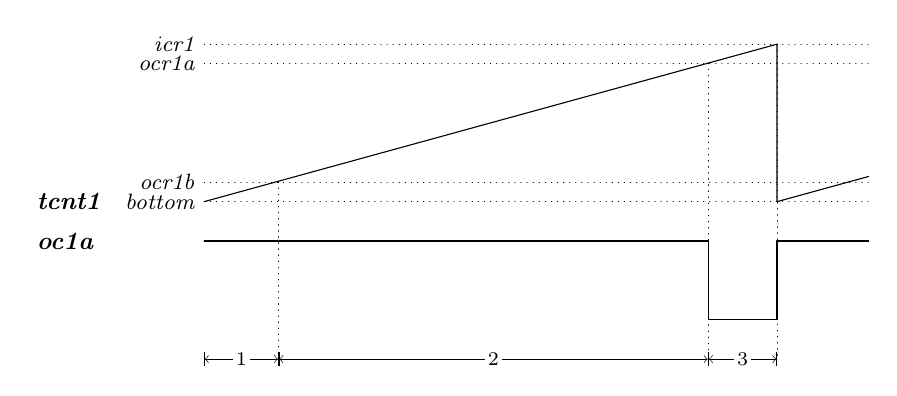
\begin{tikzpicture}[line cap = round, line join = round, quotas/.style={very thin, |<->|}]
        %
        \def\Period{0.6\linewidth}
        \def\RampAmplitude{2.0}
        %
        \def\VericalOne{0.13 * \Period}
        \def\VericalTwo{0.88 * \Period}
        \def\VericalThree{\Period}

        % ramp
        \begin{scope}[local bounding box = ramp]
            \node [anchor = east, text width = 2cm, font = \small\itshape\bfseries] at (0, -\RampAmplitude) {tcnt1};
            \foreach \it/\txt in {0/icr1, -0.24/ocr1a, -1.75/ocr1b, -2/bottom}
            {
                \draw [very thin, dotted] (0, \it) -- ++(1.16 * \Period, 0);
                \node [anchor = east, font = \footnotesize\itshape] at (0, \it) {\txt};
            }
   
            \draw (0, -\RampAmplitude) {-- ++(\Period, \RampAmplitude) -- ++(0, -\RampAmplitude) -- ++(0.16 * \Period, 0.16 * \RampAmplitude)} ;
        \end{scope}
        % pulse
        \begin{scope}[yshift = -2.5cm, local bounding box = pulse]
            \node [anchor = east, text width = 2cm, font = \small\itshape\bfseries] at (0, 0) {oc1a};
            \draw (0, 0) {-- ++(\VericalTwo, 0) -- ++(0, -1) -- ++(\Period - \VericalTwo, 0) -- ++(0, 1) -- ++(0.16 * \Period, 0)};
        \end{scope}

        \def\lastx{0}
        \foreach[count = \i, remember = \it as \lastxit] \it/\initpos in {\VericalOne/-1.75, \VericalTwo/-0.24,\VericalThree/0}
        {
            \draw [very thin, dotted] (\it, \initpos) -- (\it,   -4);
            \draw [very thin, dotted] (\it, \initpos) -- (\it,   -4);
            \draw [quotas] (\lastxit, -4) -- node[inner sep = 1pt, fill = white, font = \scriptsize] {\i} (\it,  -4);
        }
    \end{tikzpicture}
    \caption{Funcionamento do \textit{Timer 1} (\textit{Vsync})}
    \label{fig:timer-1}
\end{figure}